\section{Examples}

\begin{frame}
\frametitle{Multi-element airfoil with large kinematics}
\framesubtitle{Prime example for embedded framework}
\begin{figure}
\setlength{\fboxsep}{\valfboxsep}%\valfboxsep=0pt
\setlength{\fboxrule}{\valfboxrule}%\valfboxrule=1pt      
\foreach \n in {1,2,3,5,6,7,8,9,10,11,12,13,14}{
\centering
\only<\n>{\fbox{\includegraphics[width=0.90\paperwidth]{/home/lukas/Desktop/project/independence/project/thesis/fig/png/multielem_euler/animation\n.jpg}}}
\only<\n>{\caption{Optimization iteration \n}}
%\only<2>{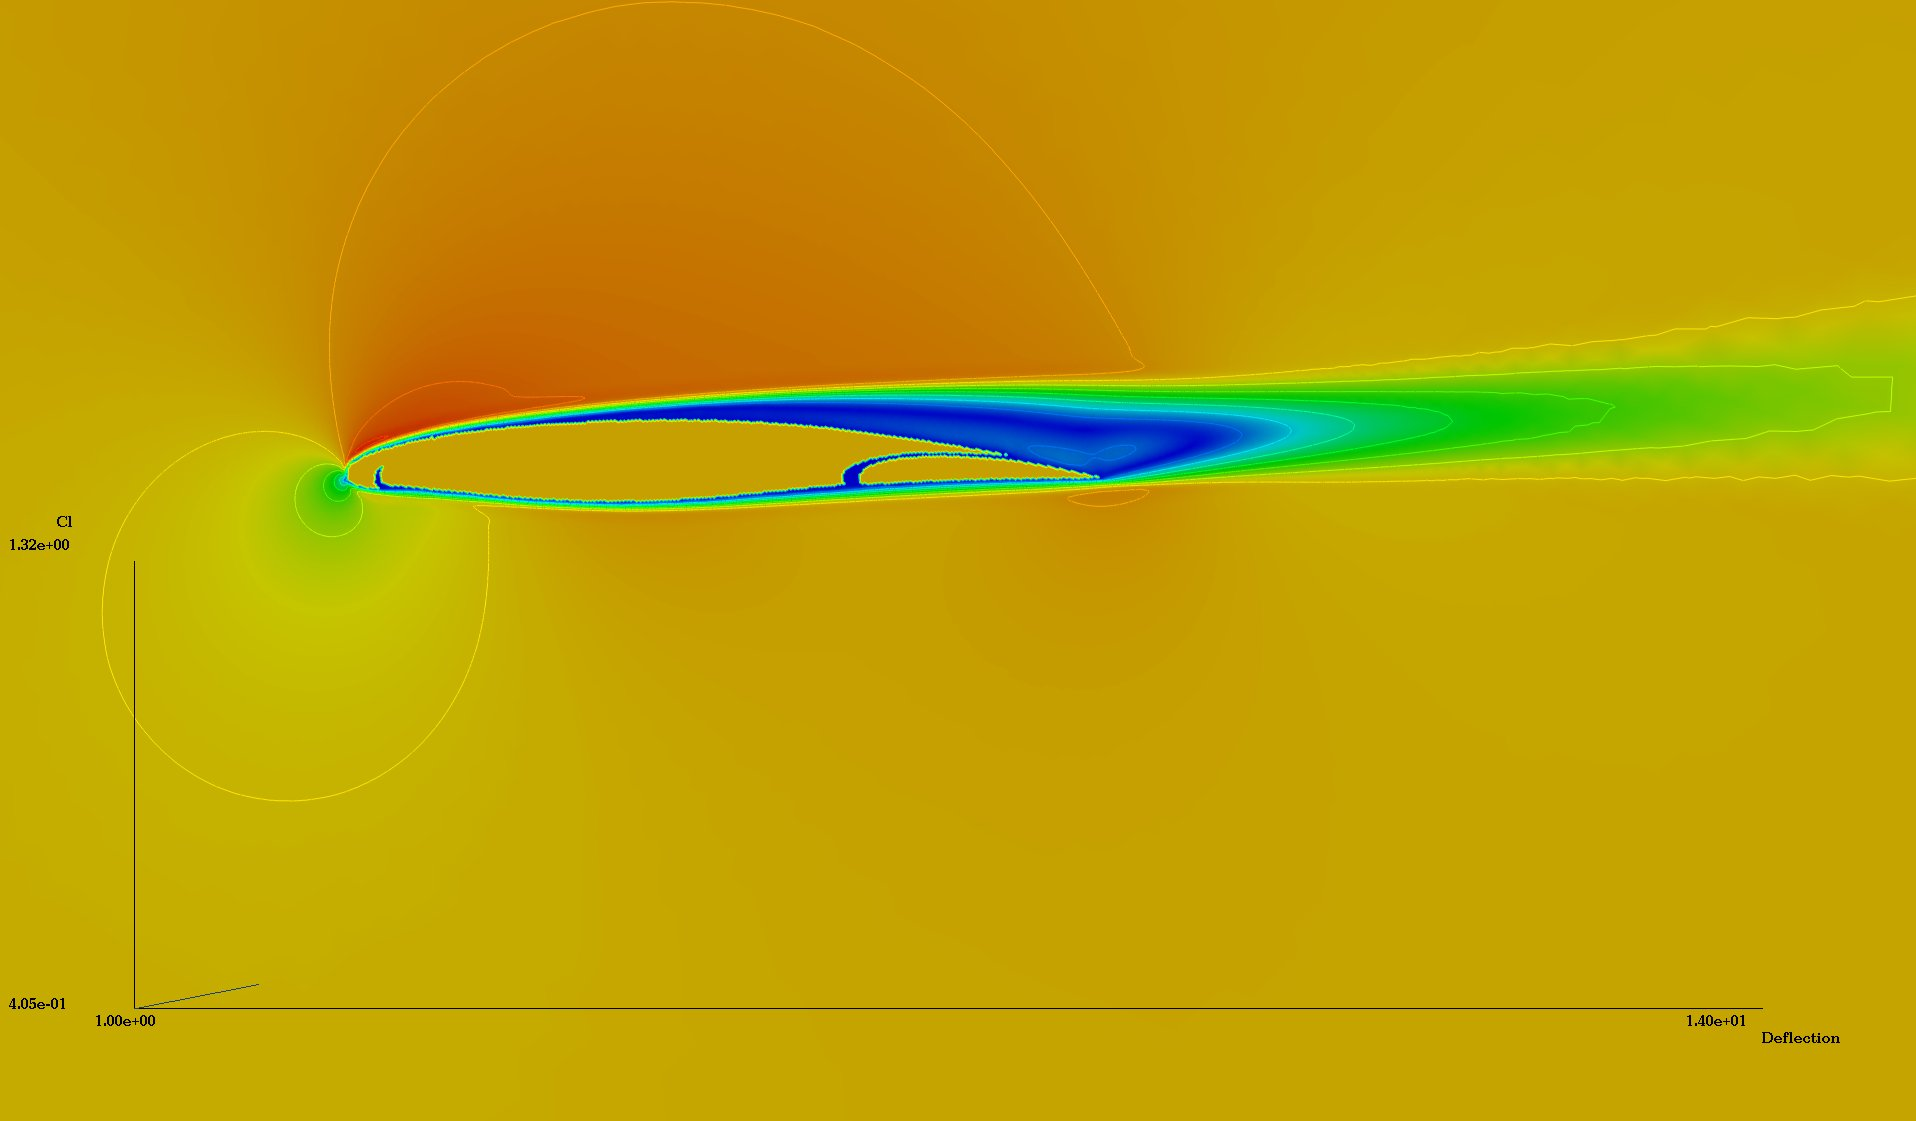
\includegraphics[width=10cm]{/home/lukas/Desktop/project/independence/project/thesis/fig/png/multielem_euler/animation2.jpg}}
}
\end{figure}
\end{frame}

%------------------------------------------------------------------------------

\begin{frame}
\frametitle{Multi-element airfoil with large kinematics}
\framesubtitle{Prime example for embedded framework}
\begin{figure}
\fbox{\includegraphics[width=0.90\paperwidth]{/home/lukas/Desktop/project/independence/Talk.d/Fig/animation_final.jpg}}
\end{figure}
\begin{itemize}
\item{$\machnum=0.2$ and $\alpha=10^{\circ}$}
\item{Starting from closed configuration; let optimizer find the best relative positions of the airfoil elements}
\item{6 design variables: rotation, vertical and horizontal displacement of the elements}
\item{Final value of the lift doubles after 6 optimization iterations}
\end{itemize}
\end{frame}